% !TEX root = ../../main.tex


\begin{figure}[!htb]
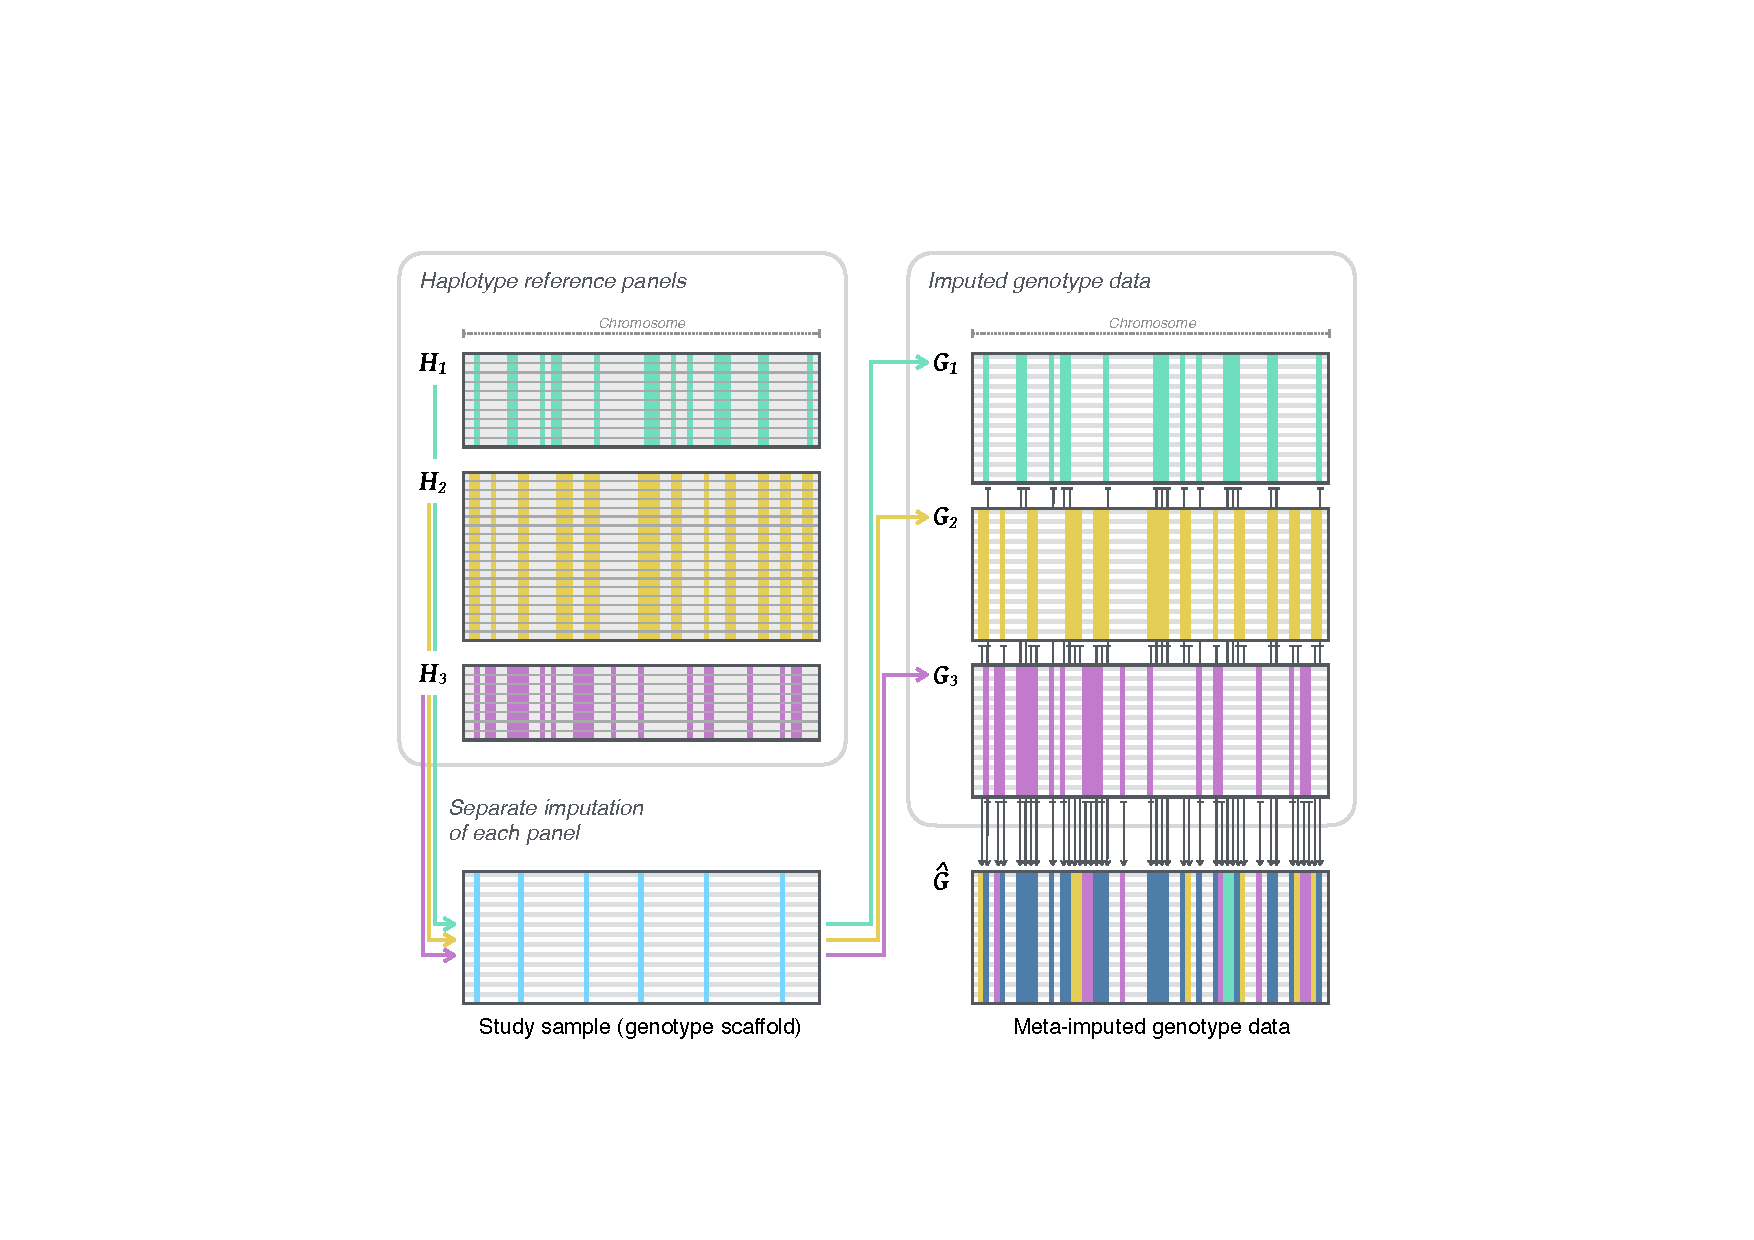
\includegraphics[width=\textwidth]{./img/ch2/info_algorithm}
\Caption{Illustration of the meta-imputation concept}
{An example of \n{3} haplotype reference panels is shown; denoted by $H_1$, $H_2$, and $H_3$, where haplotypes are indicated by row (\emph{grey}) and observed variant sites are indicated by column.
Each panel may vary in sample size and coverage.
Reference data are separately imputed into the same study sample, which is a ``scaffold'' of typed genotype markers, where individual genotypes are indicated by row (alternating \emph{grey-white}) and observed markers by column (\emph{light-blue}).
Each imputation returns an imputed genotype dataset, denoted by $G_1$, $G_2$, and $G_3$, containing marker genotypes as present in the corresponding reference panel, but where the number of individuals, $N$, is the same as in the study sample in each imputed dataset.
Imputed data are combined through meta-imputation, such that the resulting genotype dataset, $\hat{G}$, contains the union of variant sites across panels.
Variants merged across multiple datasets are indicated (\emph{dark-blue}); the markers specific to a given panel are indicated by their corresponding colour.}
{fig:info_algorithm}
\end{figure}
